% -*- latex -*-
%%%%%%%%%%%%%%%%%%%%%%%%%%%%%%%%%%%%%%%%%%%%%%%%%%%%%%%%%%%%%%%%
%%%%%%%%%%%%%%%%%%%%%%%%%%%%%%%%%%%%%%%%%%%%%%%%%%%%%%%%%%%%%%%%
%%%%
%%%% This text file is part of the lecture slides for
%%%% `Parallel Computing'
%%%% by Victor Eijkhout, copyright 2012-2020
%%%%
%%%% SPMD-slides.tex : slides about MPI's SPMD mode
%%%%
%%%%%%%%%%%%%%%%%%%%%%%%%%%%%%%%%%%%%%%%%%%%%%%%%%%%%%%%%%%%%%%%
%%%%%%%%%%%%%%%%%%%%%%%%%%%%%%%%%%%%%%%%%%%%%%%%%%%%%%%%%%%%%%%%

\begin{frame}[containsverbatim]{Overview}
  In this section you will learn how to think about parallelism in
  MPI.

  Commands learned:
  \begin{itemize}
  \item
    \indexmpishow{MPI_Init}, \indexmpishow{MPI_Finalize},
  \item 
    \indexmpishow{MPI_Get_processor_name}, \indexmpishow{MPI_Comm_size},
    \indexmpishow{MPI_Comm_rank}
  \end{itemize}
\end{frame}

\sectionframe{The MPI worldview: SPMD}

\frame{\frametitle{Computers when MPI was designed}
  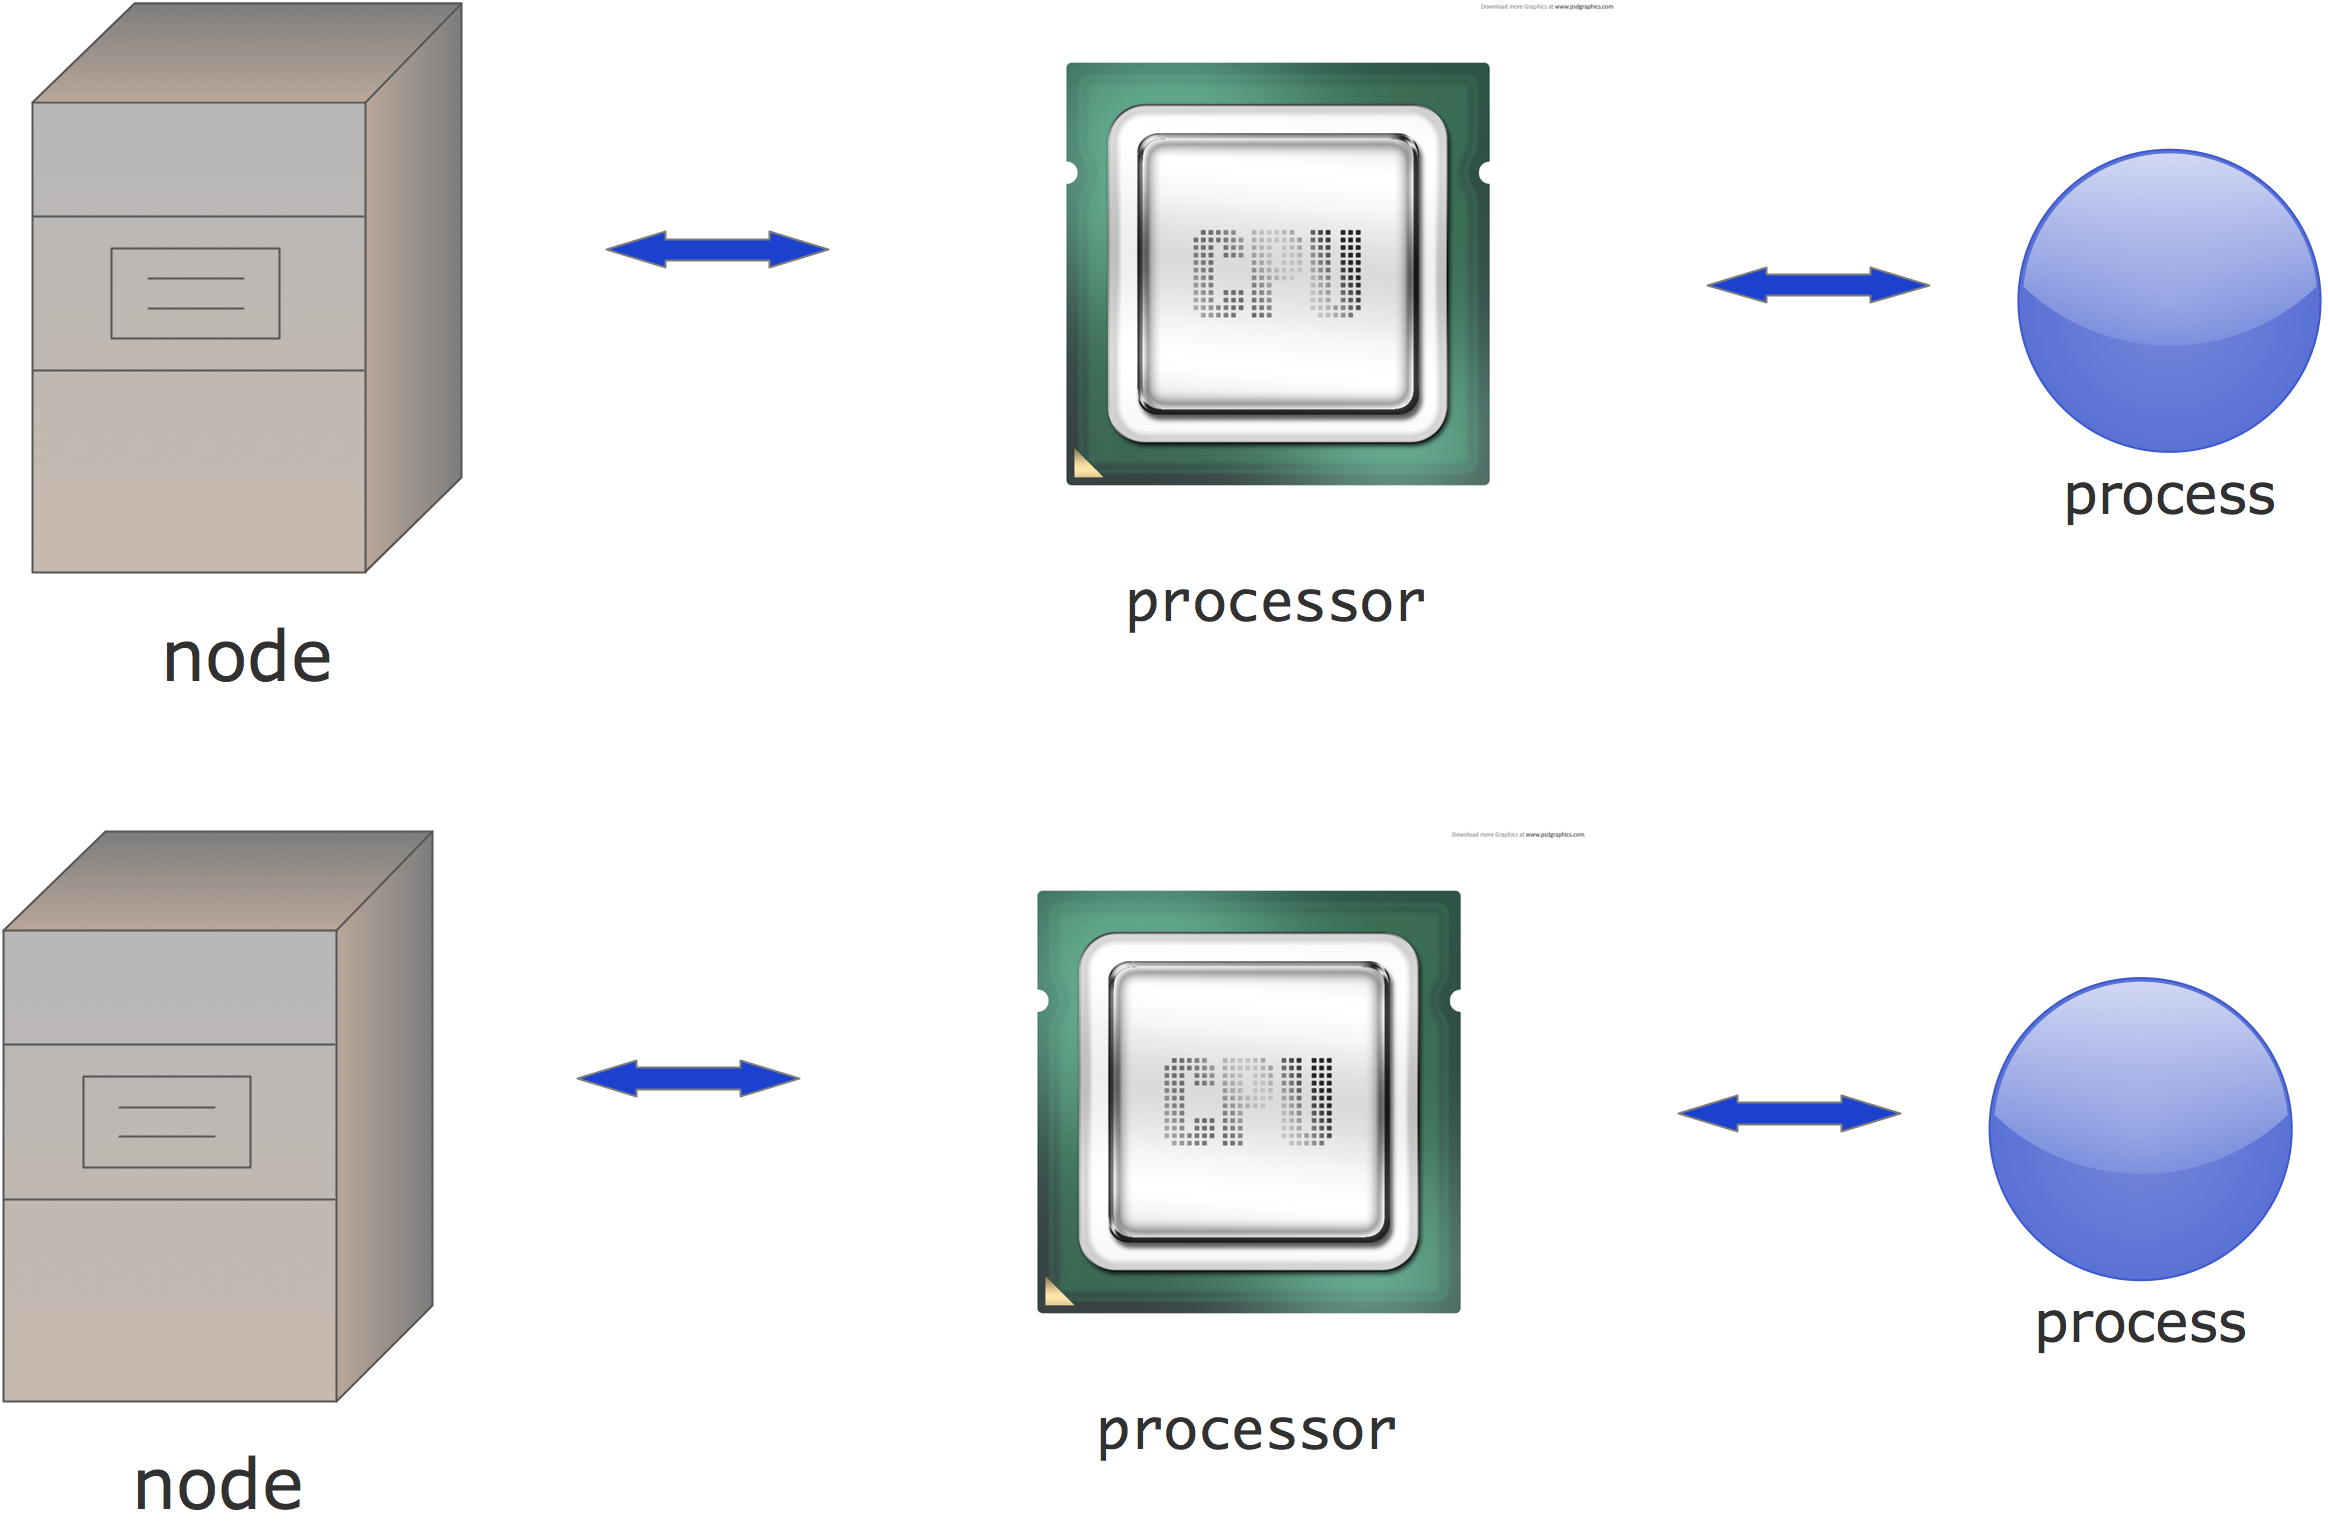
\includegraphics[scale=.1]{mpi-node1}

  One processor and one  process per node;\\
  all communication goes through the network.
}

\frame{\frametitle{Pure MPI}
  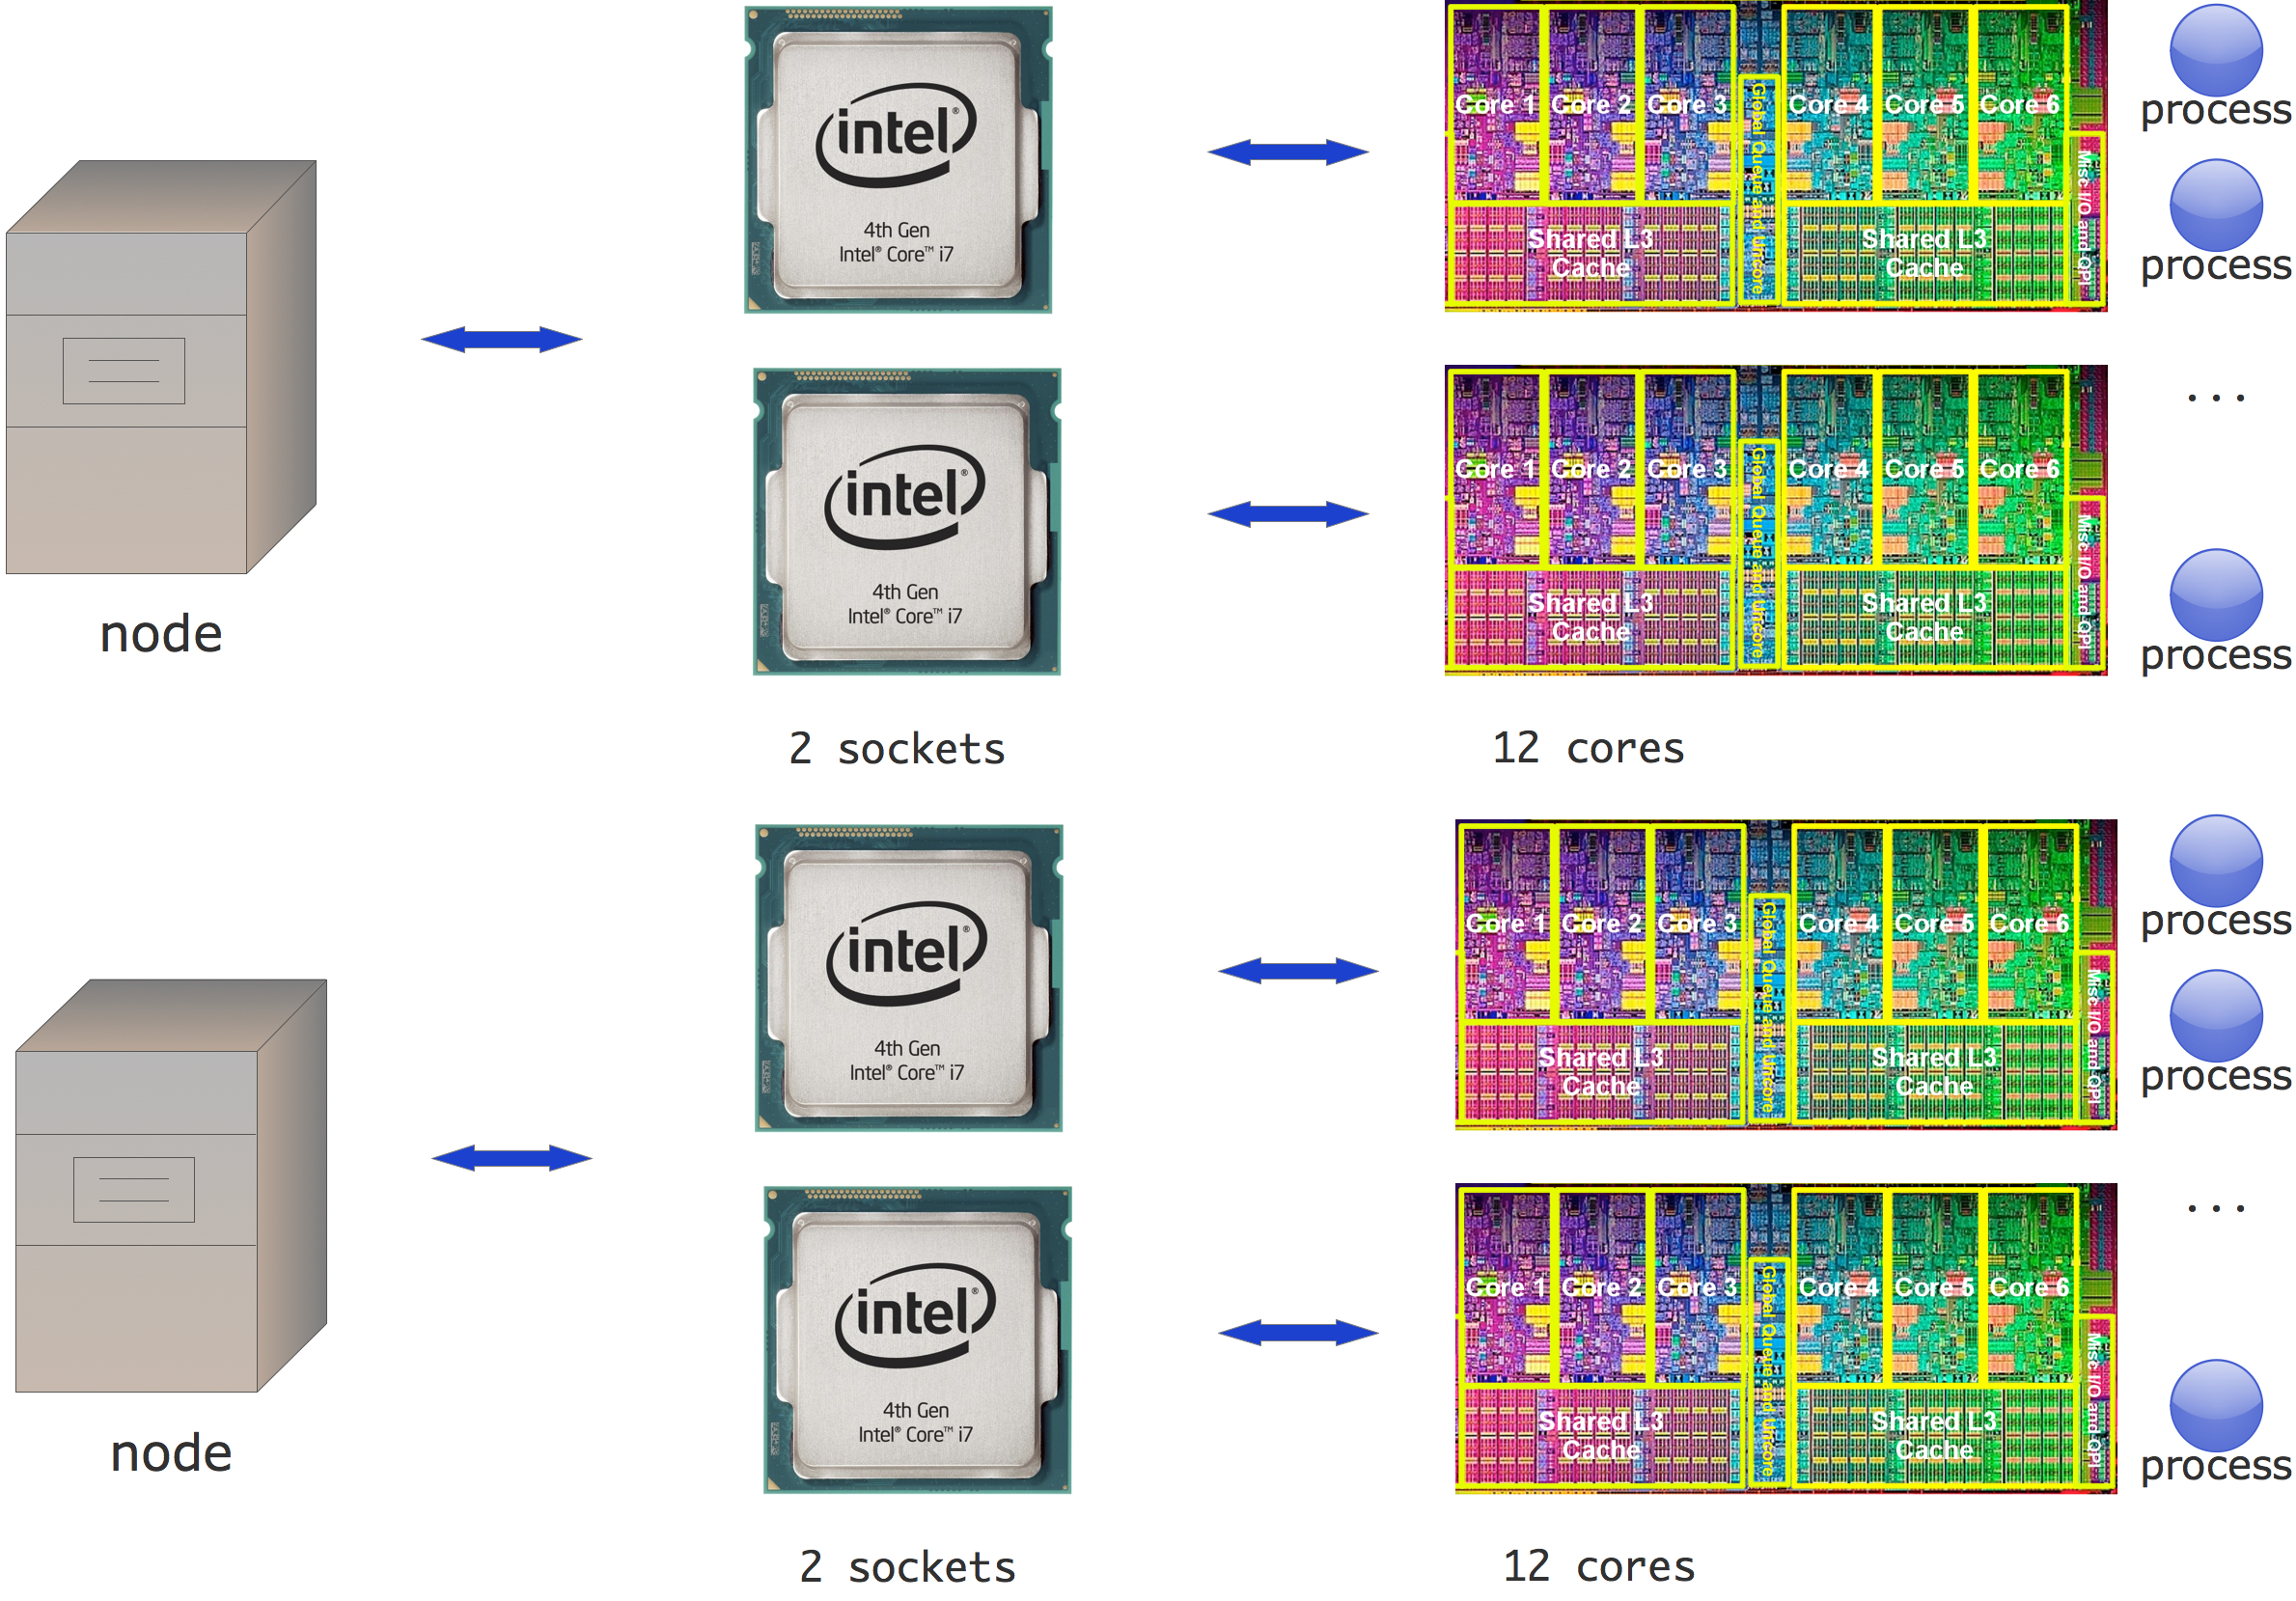
\includegraphics[scale=.1]{mpi-node2}

  A node has multiple sockets, each with multiple cores.\\
  Pure MPI puts a process on each core: pretend shared memory doesn't exist.
}

\frame{\frametitle{Hybrid programming}
  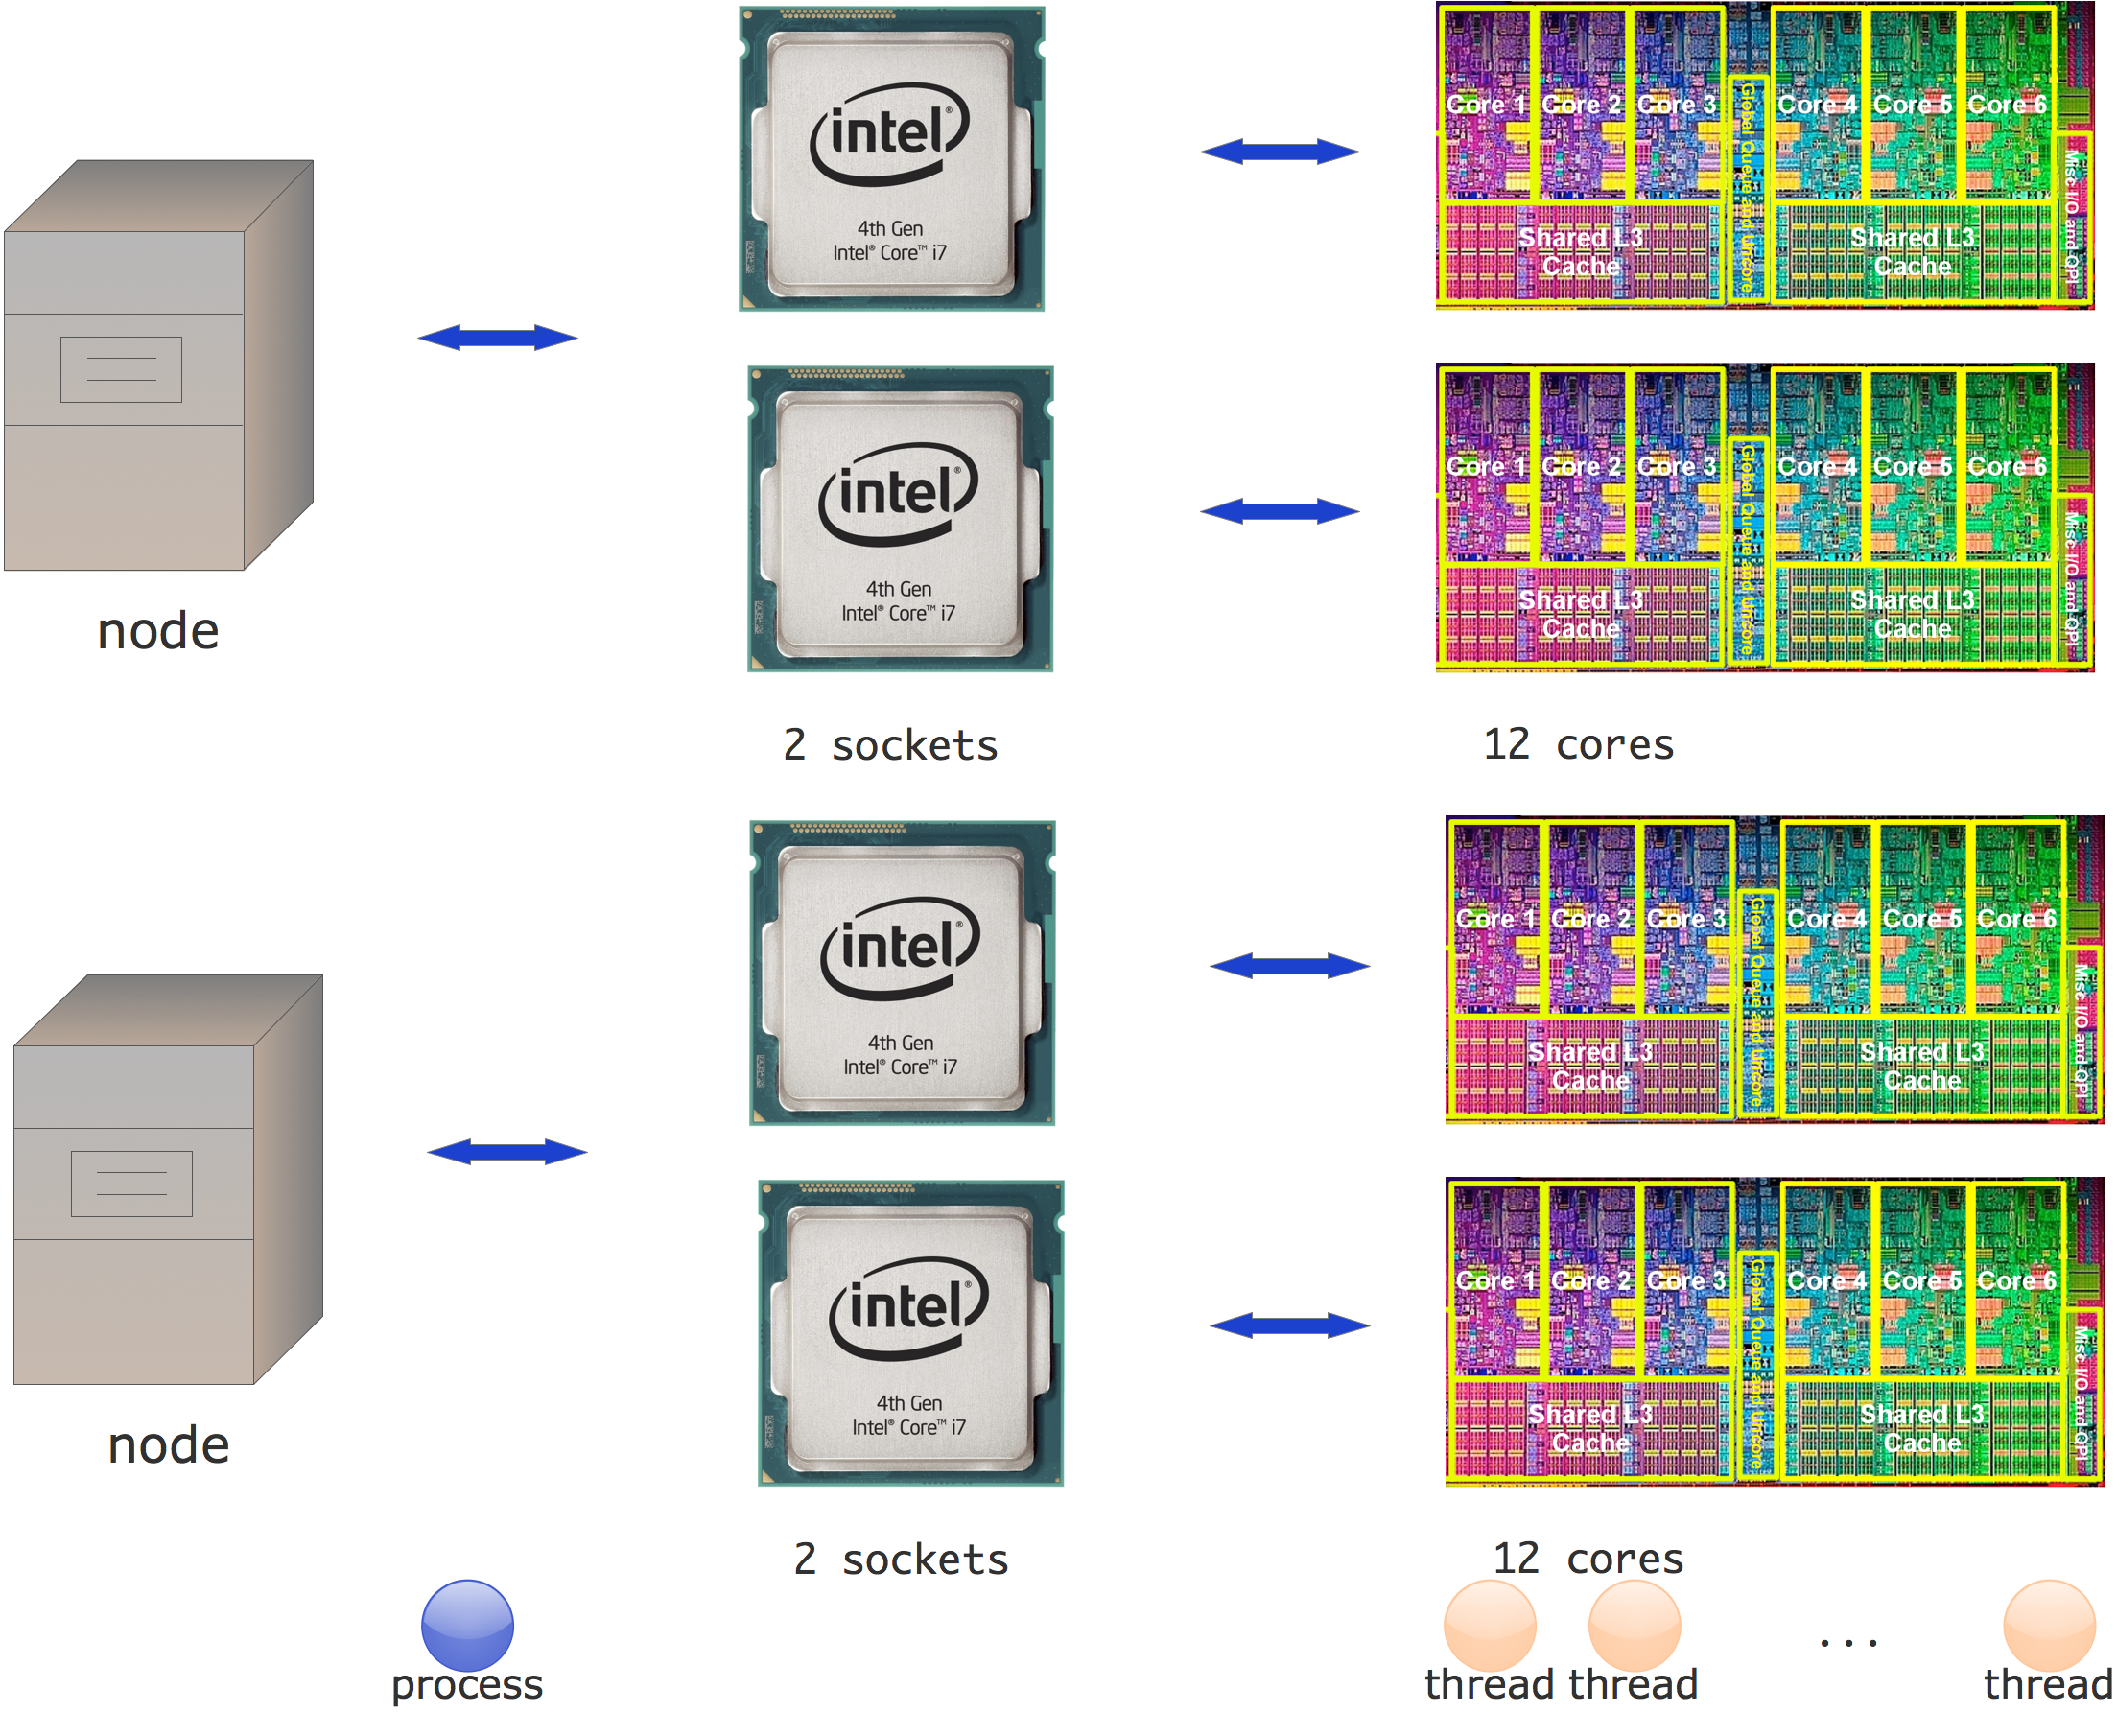
\includegraphics[scale=.1]{mpi-node3}

  Hybrid programming puts a process per node or per socket;\\
  further parallelism comes from threading.\\
  Not in this course\ldots
}

\begin{frame}{Terminology}
  `Processor' is ambiguous: is that a chip or one independent
  instruction processing unit?
  \begin{itemize}
  \item Socket: the processor chip
  \item Processor: we don't use that word
  \item Core: one instruction-stream processing unit
  \item Process: preferred terminology in talking about MPI.
  \end{itemize}  
\end{frame}

\frame{\frametitle{SPMD}
  The basic model of MPI is\\
  `Single Program Multiple Data':\\
  each process is an instance of the same program.

  Symmetry: There is no `master process', all processes are equal,
  start and end
  at the same time.

  Communication calls do not see the cluster structure:\\
  data sending/receiving is the same for all neighbours.
}

\sectionframe{Practicalities}

\begin{frame}[containsverbatim]{Compiling and running}
  MPI compilers are usually called \indextermtt{mpicc},
  \indextermtt{mpif90}, \indextermtt{mpicxx}.

  These are not separate compilers,
  but scripts around the regular C/Fortran compiler. You can use all
  the usual flags.

  Running your program:
\begin{tacc}
  At TACC:\\
  \verb+ibrun yourprog+\\
  the number of processes is determined by SLURM.
\end{tacc}
general case:
\begin{verbatim}
mpiexec -n 4 hostfile ... yourprogram arguments
mpirun -np 4 hostfile ... yourprogram arguments
\end{verbatim}
\end{frame}

\begin{frame}[containsverbatim]{Do I need a supercomputer?}
  \begin{itemize}
  \item With \n{mpiexec} and such, you start a bunch of processes that
    execute your MPI program.
  \item Does that mean that you need a cluster or a big multicore?
  \item No! You can start a large number of MPI processes, even on
    your laptop. The OS will use `time slicing'.
  \item Of course it will not be very efficient\ldots
  \end{itemize}
\end{frame}

\begin{frame}{Cluster setup}
  \small
  Typical cluster:
  \begin{itemize}
  \item Login nodes, where you ssh into; usually shared with 100 (or
    so) other people. You don't run your parallel program there!
  \item Compute nodes: where your job is run. They are often exclusive
    to you: no other users getting in the way of your program.
  \end{itemize}
  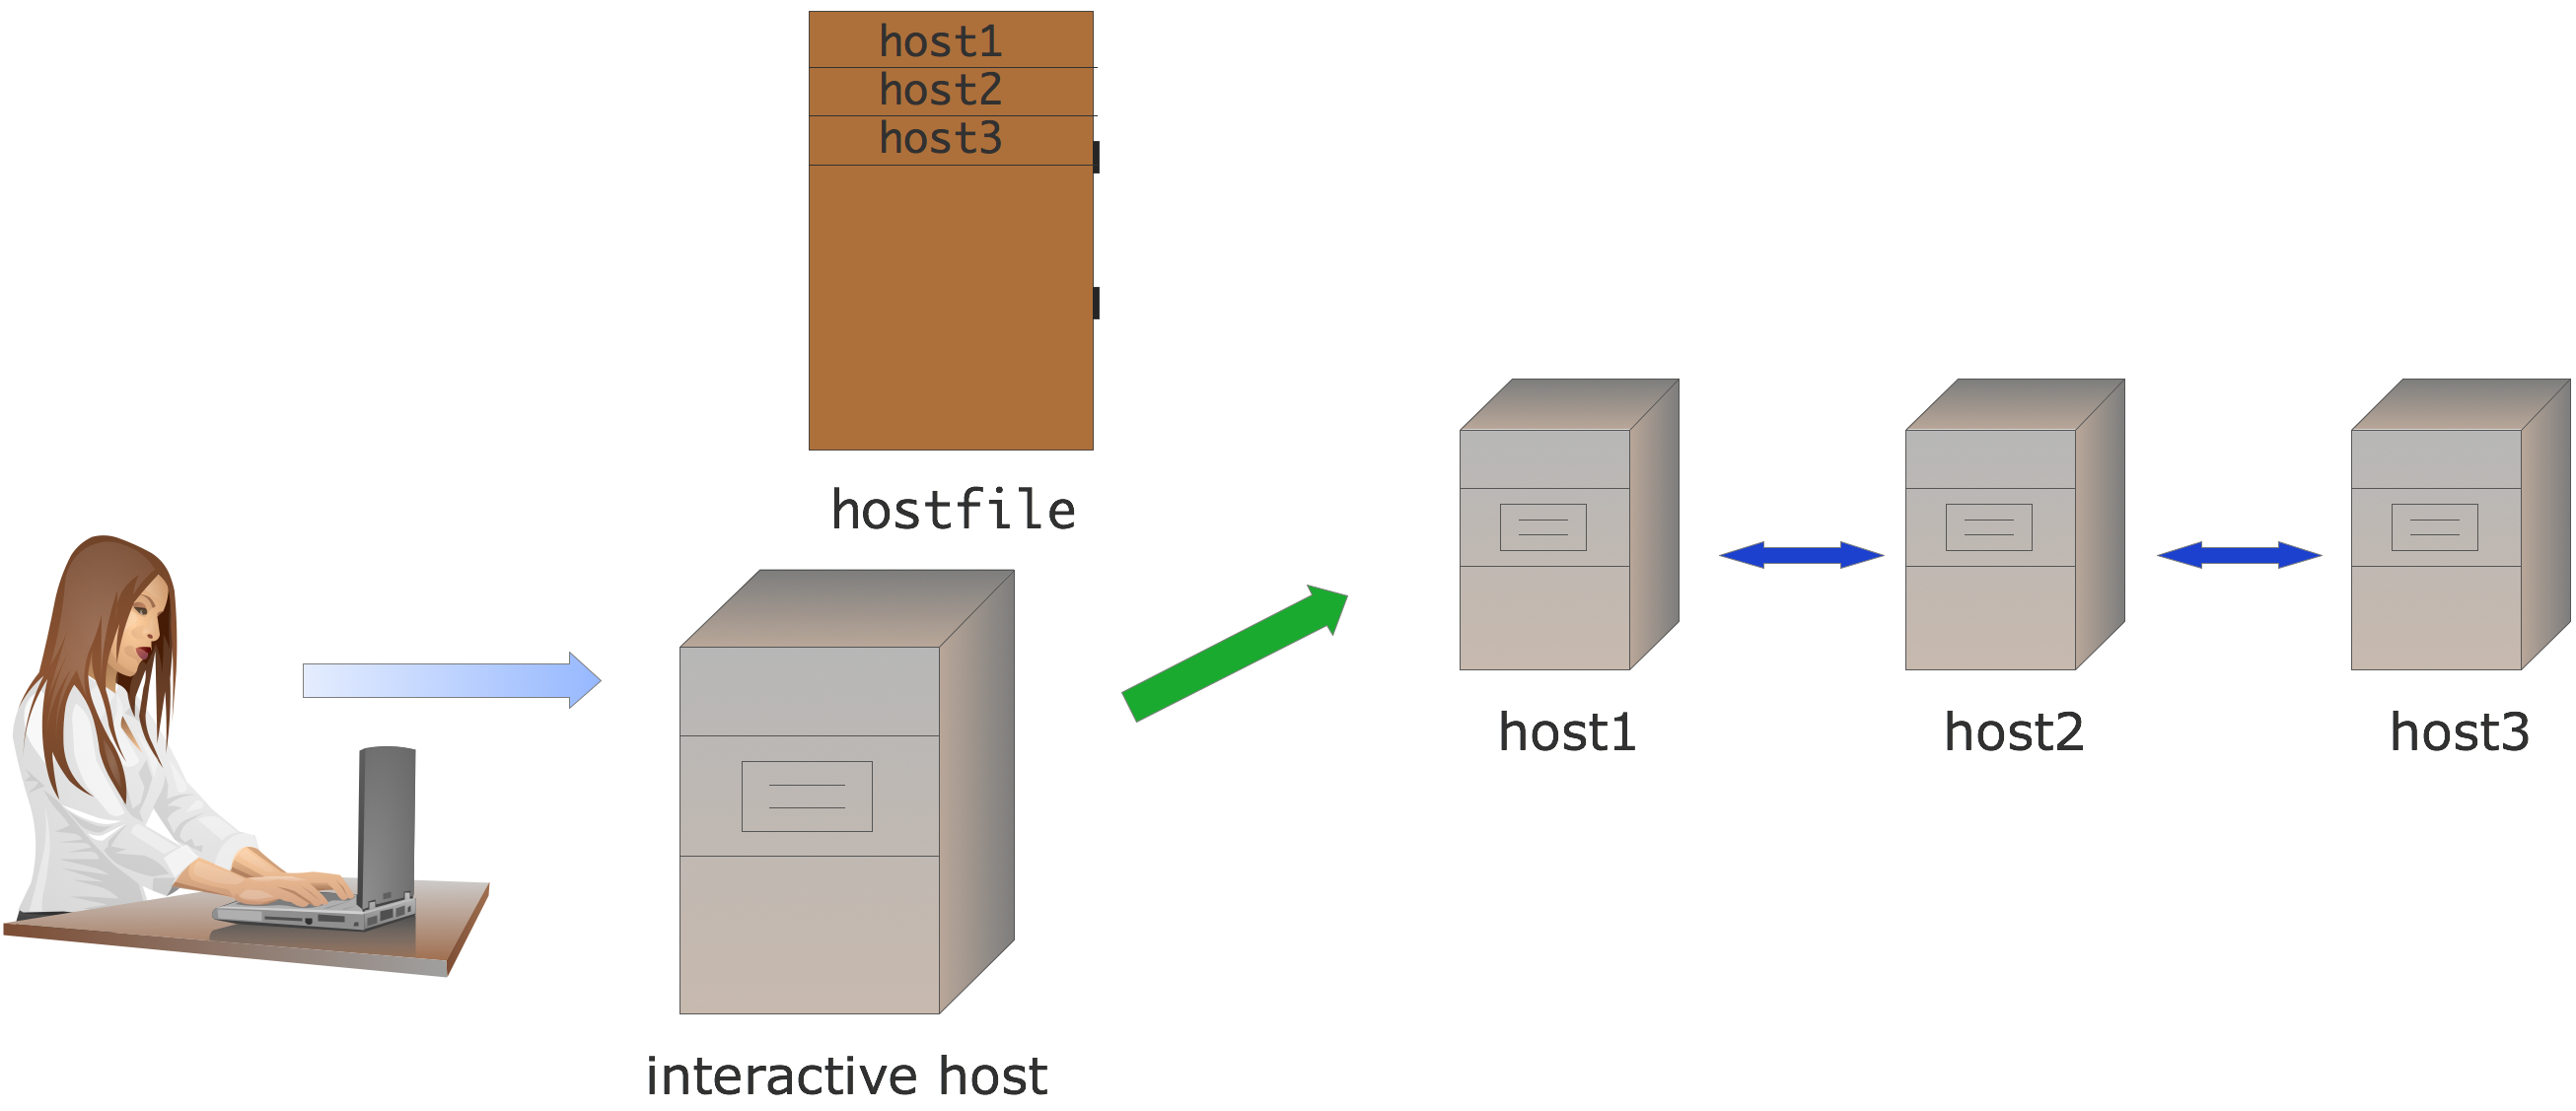
\includegraphics[scale=.08]{graphics/mpi-interactive}

  Hostfile: the description of where your job runs. Usually generated
  by a \indexterm{job scheduler}.
\end{frame}

\begin{tacc}
  \begin{frame}[containsverbatim]{Lab setup}
    \begin{itemize}
    \item Open a terminal window on a TACC cluster.
    \item Type \n{idev -N 2 -n 32 -t 4:0:0 } which gives
      you an interactive session of 2~nodes, 32~cores, for the next
      4~hours.
    \item (After this course, for serious work, you would write a
      batch script. The idev sessions are strictly limited in time and
      resources.)
    \item See the handout for reservations, project IDs, and location of training materials.
    \item Next slide for how to make and run exercises.
    \end{itemize}
  \end{frame}
\end{tacc}

\begin{frame}[containsverbatim]{How to make exercises}
  \begin{itemize}
  \item Directory: \n{exercises-mpi-c} or \n{cxx} or \n{f} or \n{f08}
    or \n{p}
  \item If a slide has a \n{(exercisename)} over it, there will be a
    template program \n{exercisename.c} (or \n{F90} or \n{py}).
  \item Type \n{make exercisename} to compile it
  \item Python: setup once per session
\begin{verbatim}
module load python3 # or python2
\end{verbatim}
No compilation needed. Run:
\begin{verbatim}
ibrun python3 yourprogram.py # or python3
\end{verbatim}
\item Add an exercise of your own to the makefile: add the name to
    the \n{EXERCISES}
  \end{itemize}
\end{frame}

\begin{exerciseframe}[hello]
  \input ex:hello1
\end{exerciseframe}

\begin{frame}{In a picture}
  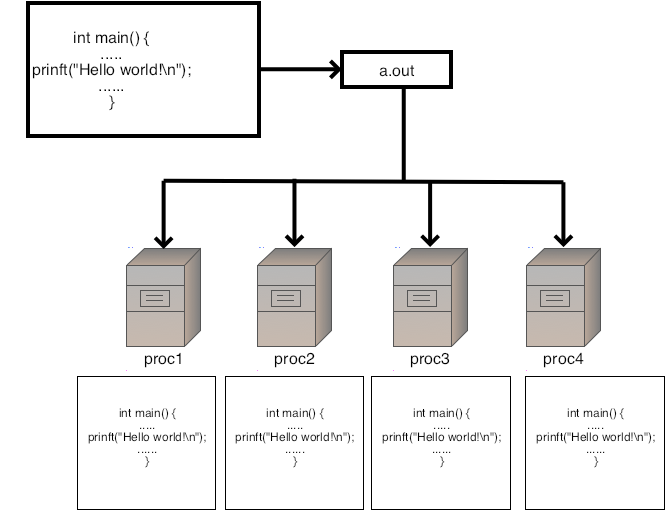
\includegraphics[scale=.35]{hello-parallel}
\end{frame}

\sectionframe{We start learning MPI!}

\begin{mpithree}
\begin{frame}[containsverbatim]{MPI definitions}
\label{sl:mpi-header}
You need an include file:
\begin{verbatim}
#include "mpi.h" // for C
use mpi_f08   ! for Fortran2008
use mpi       ! for legacy Fortran90
\end{verbatim}
\begin{itemize}
\item There are no real C++ bindings.
\item True Fortran bindings as of the 2008 standard.
\begin{tacc}
Provided in Intel compiler:
\begin{verbatim}
module load intel/18.0.2
\end{verbatim}
or newer. Not in gcc7.
\end{tacc}
(Legacy bindings are far inferior)
\end{itemize}
\end{frame}

\begin{frame}[containsverbatim]{MPI Init / Finalize}
Then put these calls around your code:
\lstset{language=C}
\begin{lstlisting}
ierr = MPI_Init(&argc,&argv); // zeros allowed
// your code
ierr = MPI_Finalize();  
\end{lstlisting}
and for Fortran:
\lstset{language=Fortran}
\begin{lstlisting}
call MPI_Init()     ! F08 style
! your code
call MPI_Finalize()

call MPI_Init(ierr) ! F90 style
! your code
call MPI_Finalize(ierr)
\end{lstlisting}
\end{frame}
\end{mpithree}

\begin{frame}{About error codes}
  MPI routines return an integer error code
  \begin{itemize}
  \item In C: function result. Can be ignored.
  \item In Fortran: as optional (F08 only) parameter.
  \item In Python: throwing exception.
  \end{itemize}
  There's actually not a lot you can do with an error code:\\
  very hard to recover from errors in parallel.\\
  Just ignore them~\ldots
\end{frame}

\begin{frame}[containsverbatim]{Python bindings}
\begin{verbatim}
module load python # or python2 or python3
\end{verbatim}
\begin{verbatim}
from mpi4py import MPI
\end{verbatim}
Run:
\begin{tacc}
\begin{verbatim}
ibrun python yourprogram.py # or python2 or python3
\end{verbatim}
\end{tacc}
\begin{verbatim}
mpiexec -n 15 python yourprogram.py
\end{verbatim}
No initialization needed.
\end{frame}

\begin{frame}[containsverbatim]{C++ bindings}
  MPI-1 had C++ bindings, by MPI-2 they were deprecated, in MPI-3 they have been removed.
  \begin{itemize}
  \item Easy solution: use the C~bindings unaltered.
    \begin{itemize}
    \item This is done in the \n{cxx} exercise directory.
    \item Ugly: very un-OO.
    \end{itemize}
  \item There are C++ bindings in Boost. No longer developed?
  \item Try MPL: \url{https://github.com/rabauke/mpl}
    \begin{itemize}
    \item Very modern OO.
    \item Exercises in \n{mpl} directory.
    \item Caution: not a full MPI implementation\\
      (I/O and one-sided mostly missing)
    \end{itemize}
  \end{itemize}
\end{frame}

\begin{exerciseframe}[hello]
  \input ex:hello2
\end{exerciseframe}

\begin{frame}[containsverbatim]\frametitle{Process identification}
Every process has a number (with respect to a communicator)
\lstset{language=C}
\begin{lstlisting}
int MPI_Comm_rank( MPI_Comm comm, int *procno )
int MPI_Comm_size( MPI_Comm comm, int *nprocs )
\end{lstlisting}
Lowest number is always zero.

For now, the communicator will be \indexmpishow{MPI_COMM_WORLD}.

Note: mapping of ranks to actual processes and cores is not predictable!
\end{frame}

\begin{frame}
  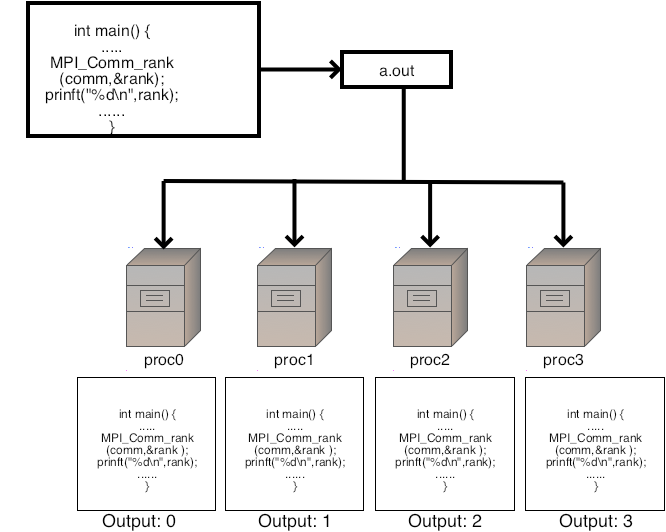
\includegraphics[scale=.35]{rank-parallel}
\end{frame}

\begin{frame}[containsverbatim]{About routine prototypes: C/C++}
  \label{sec:protos}
Prototype:
\lstset{language=C}
\begin{lstlisting}
int MPI_Comm_size(MPI_Comm comm,int *nprocs)
\end{lstlisting}
Use:
\lstset{language=C}
\begin{lstlisting}
MPI_Comm comm = MPI_COMM_WORLD;
int nprocs;
int errorcode;
errorcode = MPI_Comm_size( comm,&nprocs );
\end{lstlisting}
(but forget about that error code most of the time)
\end{frame}

\begin{mpithree}
\begin{frame}[containsverbatim]{About routine prototypes: Fortran}
Prototype
\lstset{language=Fortran}
\begin{lstlisting}
MPI_Comm_size(comm, size, ierror)
Type(MPI_Comm), INTENT(IN) :: comm
INTEGER, INTENT(OUT) :: size
INTEGER, OPTIONAL, INTENT(OUT) :: ierror
\end{lstlisting}
F90 differences:
\begin{lstlisting}
Integer, INTENT(IN) :: comm
INTEGER, OPTIONAL :: ierror
\end{lstlisting}
Use:
\begin{lstlisting}
Type(MPI_Comm) :: comm = MPI_COMM_WORLD
integer :: size
CALL MPI_Comm_size( comm, size, ierr ) ! F90 style
CALL MPI_Comm_size( comm, size ) ! F2008 style
\end{lstlisting}
\begin{itemize}
\item Fortran2008: final parameter optional.
\item Fortran90: final parameter always error parameter. Do not
  forget!
\item Fortran2008: \n{MPI_...} types are \n{Type}.
\item Fortran90: \n{MPI_...} types are \n{INTEGER}.
\end{itemize}
\end{frame}
\end{mpithree}

\begin{frame}[containsverbatim]{About routine prototypes: Python}
Prototype:
\lstset{language=Python}
\begin{lstlisting}
# object method
MPI.Comm.Send(self, buf, int dest, int tag=0)
# class method
MPI.Request.Waitall(type cls, requests, statuses=None)
\end{lstlisting}
Use:
\begin{lstlisting}
from mpi4py import MPI
comm = MPI.COMM_WORLD
comm.Send(sendbuf,dest=other)
MPI.Request.Waitall(requests)
\end{lstlisting}
Note: most functions are methods of the \lstinline{MPI.Comm} class.\\
(Sometimes of \lstinline{MPI}, sometimes other.)
\end{frame}

\protoslide{MPI_Comm_size}
\protoslide{MPI_Comm_rank}

\begin{frame}{Have you been paying attention?}
  \input{ex:mpi01rank}
\end{frame}

\begin{exerciseframe}[commrank]
  \input ex:hello3
\end{exerciseframe}

\begin{exerciseframe}[commrank]
  \input ex:hello4
\end{exerciseframe}

\begin{optexerciseframe}
  \input ex:procname
\end{optexerciseframe}

\protoslide{MPI_Get_processor_name}

\begin{frame}{In a picture}
  Four processes on two nodes (\n{idev -N 2 -n 4})
  
\includegraphics[scale=.3]{node-comm-rank}
\end{frame}

\sectionframe{A practical example}

\begin{frame}{Functional Parallelism}
  Parallelism by letting each process do a different thing.

  Example: divide up a search space.

  Each process knows its rank, so it can find its part of the search space.
\end{frame}

\begin{exerciseframe}[prime]
  \input ex:primetest
\end{exerciseframe}

\endinput

\begin{frame}[containsverbatim]\frametitle{}
\begin{lstlisting}
  
\end{lstlisting}
\end{frame}

